% generated by Plantuml 1.2025.0       
\definecolor{plantucolor0000}{RGB}{0,0,0}
\definecolor{plantucolor0001}{RGB}{241,241,241}
\definecolor{plantucolor0002}{RGB}{24,24,24}
\definecolor{plantucolor0003}{RGB}{254,255,221}
\definecolor{plantucolor0004}{RGB}{255,0,0}
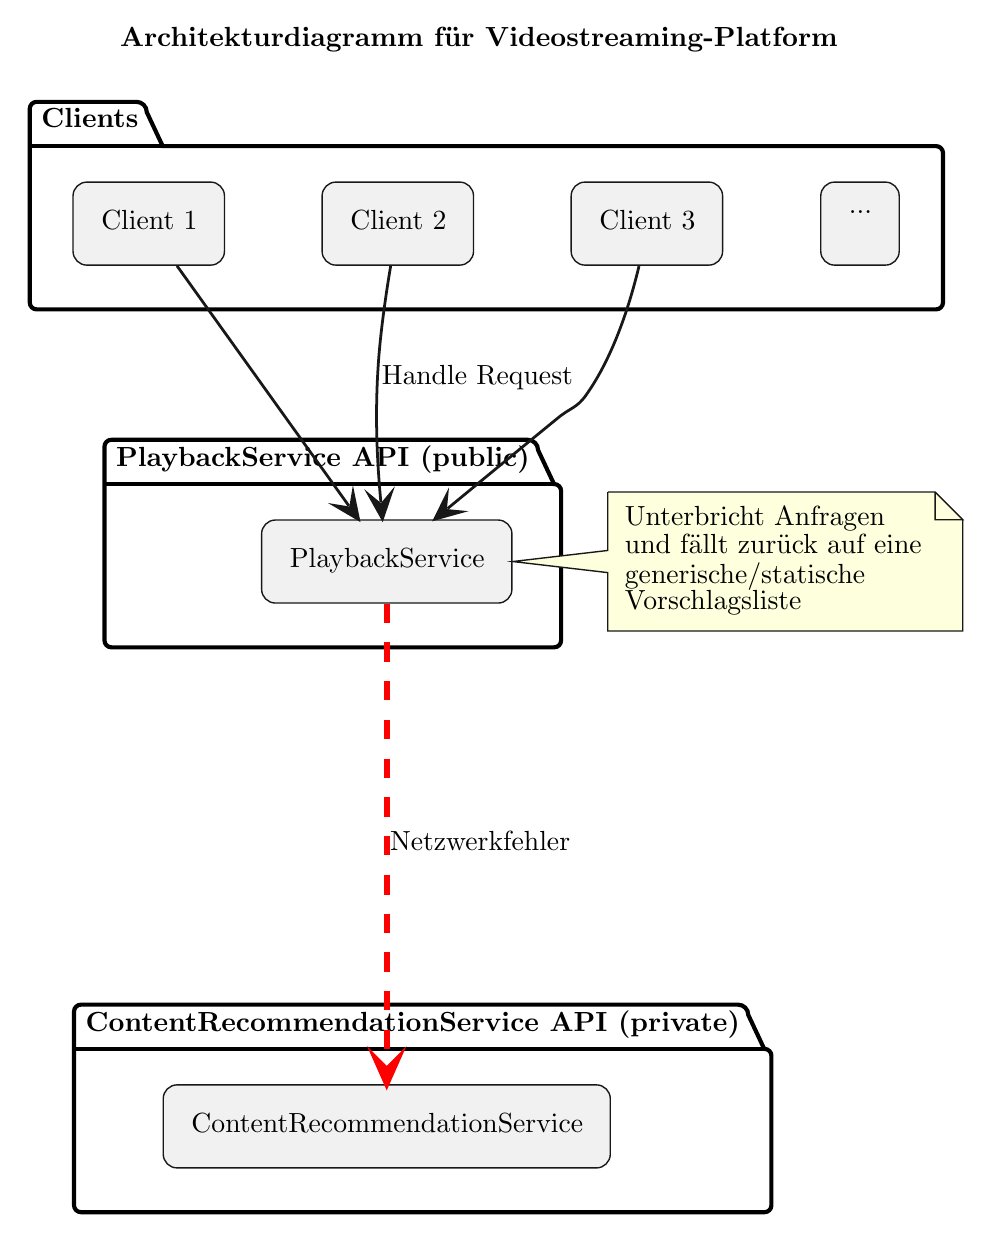
\begin{tikzpicture}[yscale=-1
,pstyle0/.style={color=black,line width=1.5pt}
,pstyle1/.style={color=plantucolor0002,fill=plantucolor0001,line width=0.5pt}
,pstyle2/.style={color=plantucolor0002,fill=plantucolor0003,line width=0.5pt}
,pstyle3/.style={color=plantucolor0002,line width=1.0pt}
,pstyle4/.style={color=plantucolor0002,fill=plantucolor0002,line width=1.0pt}
]
\node at (38.44pt,10pt)[below right,color=black,inner sep=0]{\textbf{Architekturdiagramm für Videostreaming-Platform}};
\draw[pstyle0] (8.5pt,37pt) -- (44.54pt,37pt) arc(270:360:3.75pt)  -- (54.04pt,53pt) -- (333.5pt,53pt) arc(270:360:2.5pt)  -- (336pt,109.5pt) arc(0:90:2.5pt)  -- (8.5pt,112pt) arc(90:180:2.5pt)  -- (6pt,39.5pt) arc(180:270:2.5pt) ;
\draw[pstyle0] (6pt,53pt) -- (54.04pt,53pt);
\node at (10pt,39pt)[below right,color=black,inner sep=0]{\textbf{Clients}};
\draw[pstyle0] (35.5pt,159.11pt) -- (185.94pt,159.11pt) arc(270:360:3.75pt)  -- (195.44pt,175.11pt) -- (195.5pt,175.11pt) arc(270:360:2.5pt)  -- (198pt,231.61pt) arc(0:90:2.5pt)  -- (35.5pt,234.11pt) arc(90:180:2.5pt)  -- (33pt,161.61pt) arc(180:270:2.5pt) ;
\draw[pstyle0] (33pt,175.11pt) -- (195.44pt,175.11pt);
\node at (37pt,161.11pt)[below right,color=black,inner sep=0]{\textbf{PlaybackService API (public)}};
\draw[pstyle0] (24.5pt,363.22pt) -- (261.9pt,363.22pt) arc(270:360:3.75pt)  -- (271.4pt,379.22pt) -- (271.5pt,379.22pt) arc(270:360:2.5pt)  -- (274pt,435.72pt) arc(0:90:2.5pt)  -- (24.5pt,438.22pt) arc(90:180:2.5pt)  -- (22pt,365.72pt) arc(180:270:2.5pt) ;
\draw[pstyle0] (22pt,379.22pt) -- (271.4pt,379.22pt);
\node at (26pt,365.22pt)[below right,color=black,inner sep=0]{\textbf{ContentRecommendationService API (private)}};
\draw[pstyle1] (21.64pt,71pt) arc (180:270:5pt) -- (26.64pt,66pt) -- (71.36pt,66pt) arc (270:360:5pt) -- (76.36pt,71pt) -- (76.36pt,91pt) arc (0:90:5pt) -- (71.36pt,96pt) -- (26.64pt,96pt) arc (90:180:5pt) -- (21.64pt,91pt) -- cycle;
\node at (31.64pt,76pt)[below right,color=black,inner sep=0]{Client 1};
\draw[pstyle1] (111.64pt,71pt) arc (180:270:5pt) -- (116.64pt,66pt) -- (161.36pt,66pt) arc (270:360:5pt) -- (166.36pt,71pt) -- (166.36pt,91pt) arc (0:90:5pt) -- (161.36pt,96pt) -- (116.64pt,96pt) arc (90:180:5pt) -- (111.64pt,91pt) -- cycle;
\node at (121.64pt,76pt)[below right,color=black,inner sep=0]{Client 2};
\draw[pstyle1] (201.64pt,71pt) arc (180:270:5pt) -- (206.64pt,66pt) -- (251.36pt,66pt) arc (270:360:5pt) -- (256.36pt,71pt) -- (256.36pt,91pt) arc (0:90:5pt) -- (251.36pt,96pt) -- (206.64pt,96pt) arc (90:180:5pt) -- (201.64pt,91pt) -- cycle;
\node at (211.64pt,76pt)[below right,color=black,inner sep=0]{Client 3};
\draw[pstyle1] (291.83pt,71pt) arc (180:270:5pt) -- (296.83pt,66pt) -- (315.17pt,66pt) arc (270:360:5pt) -- (320.17pt,71pt) -- (320.17pt,91pt) arc (0:90:5pt) -- (315.17pt,96pt) -- (296.83pt,96pt) arc (90:180:5pt) -- (291.83pt,91pt) -- cycle;
\node at (301.83pt,76pt)[below right,color=black,inner sep=0]{...};
\draw[pstyle1] (89.78pt,193.11pt) arc (180:270:5pt) -- (94.78pt,188.11pt) -- (175.23pt,188.11pt) arc (270:360:5pt) -- (180.23pt,193.11pt) -- (180.23pt,213.11pt) arc (0:90:5pt) -- (175.23pt,218.11pt) -- (94.78pt,218.11pt) arc (90:180:5pt) -- (89.78pt,213.11pt) -- cycle;
\node at (99.78pt,198.11pt)[below right,color=black,inner sep=0]{PlaybackService};
\draw[pstyle1] (54.23pt,397.22pt) arc (180:270:5pt) -- (59.23pt,392.22pt) -- (210.78pt,392.22pt) arc (270:360:5pt) -- (215.78pt,397.22pt) -- (215.78pt,417.22pt) arc (0:90:5pt) -- (210.78pt,422.22pt) -- (59.23pt,422.22pt) arc (90:180:5pt) -- (54.23pt,417.22pt) -- cycle;
\node at (64.23pt,402.22pt)[below right,color=black,inner sep=0]{ContentRecommendationService};
\draw[pstyle2] (214.86pt,178pt) -- (214.86pt,199.11pt) -- (180.56pt,203.11pt) -- (214.86pt,207.11pt) -- (214.86pt,228.22pt) -- (214.86pt,228.22pt) -- (343.13pt,228.22pt) -- (343.13pt,228.22pt) -- (343.13pt,188pt) -- (333.13pt,178pt) -- (214.86pt,178pt) -- (214.86pt,178pt);
\draw[pstyle2] (333.13pt,178pt) -- (333.13pt,188pt) -- (343.13pt,188pt) -- (333.13pt,178pt);
\node at (220.86pt,183pt)[below right,color=black,inner sep=0]{Unterbricht Anfragen};
\node at (220.86pt,193.22pt)[below right,color=black,inner sep=0]{und fällt zurück auf eine};
\node at (220.86pt,203.22pt)[below right,color=black,inner sep=0]{generische/statische};
\node at (220.86pt,213.22pt)[below right,color=black,inner sep=0]{Vorschlagsliste};
\draw[pstyle3] (59.2pt,96.25pt) ..controls (75.75pt,119.37pt) and (104.778pt,159.8909pt) .. (121.318pt,183.0009pt);
\draw[pstyle4] (124.81pt,187.88pt) -- (122.8247pt,178.2333pt) -- (121.9pt,183.8141pt) -- (116.3192pt,182.8893pt) -- (124.81pt,187.88pt) -- cycle;
\draw[pstyle3] (136.45pt,96.1pt) ..controls (134.81pt,105.86pt) and (132.84pt,119.17pt) .. (132pt,131pt) ..controls (130.61pt,150.6pt) and (131.5474pt,167.3055pt) .. (132.8774pt,181.6855pt);
\draw[pstyle4] (133.43pt,187.66pt) -- (136.5841pt,178.3299pt) -- (132.9695pt,182.6812pt) -- (128.6181pt,179.0666pt) -- (133.43pt,187.66pt) -- cycle;
\node at (133pt,132pt)[below right,color=black,inner sep=0]{Handle Request};
\draw[pstyle3] (226.15pt,96.35pt) ..controls (223.04pt,109.41pt) and (217.11pt,128.78pt) .. (207pt,143pt) ..controls (203.69pt,147.66pt) and (201.43pt,147.49pt) .. (197pt,151.11pt) ..controls (181.89pt,163.45pt) and (169.3894pt,173.7331pt) .. (156.9694pt,183.9731pt);
\draw[pstyle4] (152.34pt,187.79pt) -- (161.8287pt,185.151pt) -- (156.1979pt,184.6093pt) -- (156.7396pt,178.9784pt) -- (152.34pt,187.79pt) -- cycle;
\draw[color=plantucolor0004,line width=2.0pt,dash pattern=on 7.0pt off 7.0pt] (135pt,218.32pt) ..controls (135pt,255.34pt) and (135pt,348.45pt) .. (135pt,385.75pt);
\draw[color=plantucolor0004,fill=plantucolor0004,line width=2.0pt] (135pt,391.75pt) -- (139pt,382.75pt) -- (135pt,386.75pt) -- (131pt,382.75pt) -- (135pt,391.75pt) -- cycle;
\node at (136pt,300.22pt)[below right,color=black,inner sep=0]{Netzwerkfehler};
\end{tikzpicture}
